\documentclass[12pt,aspectratio=169]{beamer}
\usepackage[utf8]{inputenc}
\usepackage{amsmath}
\usepackage{mathtools}
\usepackage{amsfonts}
\usepackage{amssymb}
\usepackage{graphicx}
\usepackage{physics}
\usepackage{xcolor}
\beamertemplatenavigationsymbolsempty

\title{ Improving Quantum Gates\\ with\\ Optimal Quantum Control}
\author{\large L. Pereira, R. González, M. Á. Palomo, A. Bravo, R. Romero}
\date{}

\begin{document}
	
	\begin{frame}
		\titlepage
	\end{frame}

	\begin{frame}
		\centering
		It is necessary to improve the fidelity of quantum gates to achieve computational advantage with quantum computers. \\
		\vspace{.5cm}
		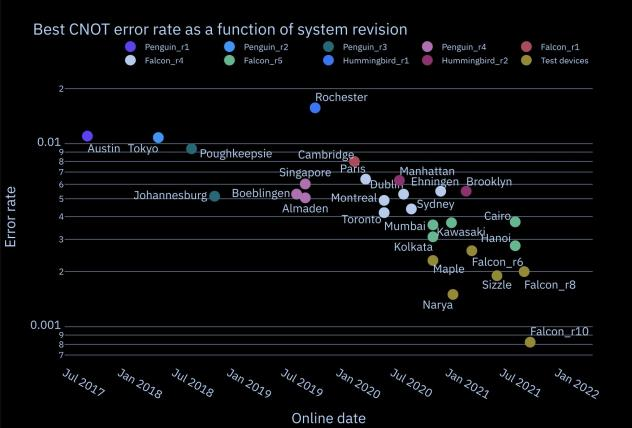
\includegraphics[scale=0.4]{cnot_ibm.jpg}\\
		{\scriptsize  https://twitter.com/jaygambetta/status/1445115380616335373 }
	\end{frame}

	\begin{frame}
		\centering
		An alternative is use optimal quantum control.\\
		\vspace{.5cm}
		$\rightarrow$ Gradient Ascent Pulse Engineering (GRAPE) Pulses.\\
		\vspace{.5cm}
		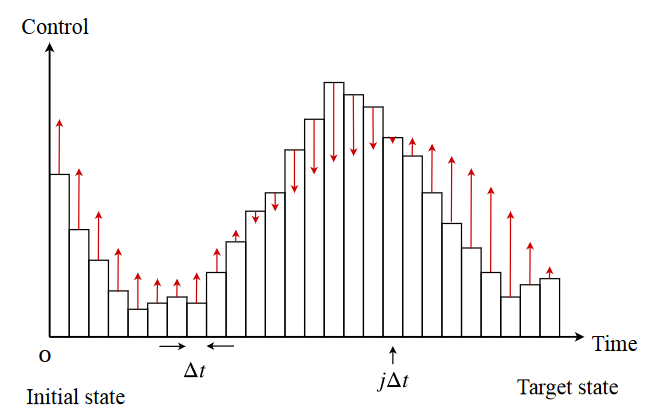
\includegraphics[scale=0.6]{grape}\\

		{\scriptsize  
		Y. Shi \emph{et al.}, "Optimized Compilation of Aggregated Instructions for Realistic Quantum Computers".}
		
	\end{frame}

	\begin{frame}
		
		\begin{minipage}{0.5\linewidth}
			We optimize the GRAPE pulse maximizing the Fidelity.
			\begin{equation*}
				f(\vec{w}) = \frac{1}{d^2} |  Tr( V^\dagger U(\vec{w})  ) |^2.
			\end{equation*}
			This can be evaluated:
			\begin{itemize}
				\item Numerically, proposing a model for the system.
				\item Experimentally. {\scriptsize S. T. Flammia and Y.-K. Liu, "Direct Fidelity Estimation from Few Pauli Measurements"}.
			\end{itemize}
		\end{minipage}%
		\begin{minipage}{0.5\linewidth}
			\centering
			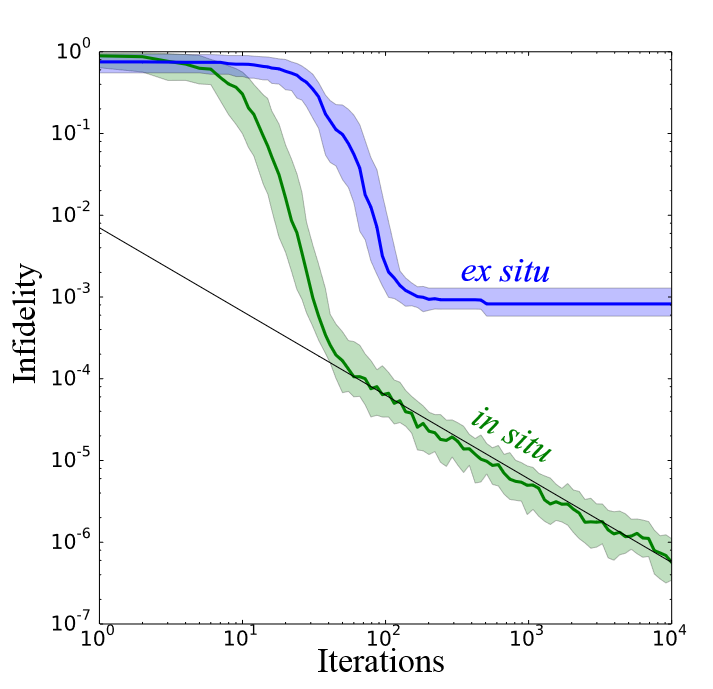
\includegraphics[scale=0.45]{fidelidad.png}\\
			{\scriptsize C. Ferrie and O. Moussa, "Robust and efficient in situ quantum control".}
		\end{minipage}
		
	\end{frame}
	
	\begin{frame}
		\begin{itemize}
			\item We build a Qiskit library to perform the ex-situ and in-situ quantum control with GRAPE.\\
			\vspace{0.1cm}
			\item We implement GRAPE pulses with Qiskit Pulse.
			\vspace{0.1cm}
			\item We implement Direct Fidelity Estimation for unitary gates.
			\vspace{0.1cm}
			\item We propose a mixed protocol, where first the ex-situ quantum control is carried out, to then refine the result with in-situ quantum control.\\
			\vspace{0.1cm}
			\item We implement the not-gate with ex-situ and in-situ quantum control.
		\end{itemize}
		
	\end{frame}
	
	\begin{frame}
		\centering
		\includegraphics[scale=0.8]{infidelity.png}
	\end{frame}
	
	\begin{frame}
		\centering
		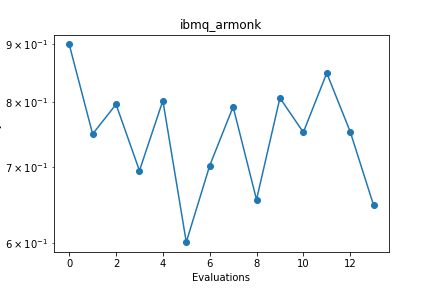
\includegraphics[scale=0.8]{experiment.png}
	\end{frame}
	
	
\end{document}















